% ------------------------------------------------------------------------------
% TYPO3 CMS 7.0 - What's New - Chapter "Introduction" (Russian Version)
%
% @author	Michael Schams <schams.net>
% @license	Creative Commons BY-NC-SA 3.0
% @link		http://typo3.org/download/release-notes/whats-new/
% @language	Russian
% ------------------------------------------------------------------------------
% LTXE-CHAPTER-UID:		a1b460e2-d97f2dc7-79fb6415-08d6615b
% LTXE-CHAPTER-NAME:	Introduction
% ------------------------------------------------------------------------------

\section{Введение}
\begin{frame}[fragile]
	\frametitle{Введение}

	\begin{center}\huge{Введение}\end{center}
	\begin{center}\huge{\color{typo3darkgrey}\textbf{Факты}}\end{center}

\end{frame}

% ------------------------------------------------------------------------------
% LTXE-SLIDE-START
% LTXE-SLIDE-UID:		9e930c22-df341073-f0b4f378-8764212a
% LTXE-SLIDE-ORIGIN:	c0dd5662-b64f5b3d-ea39556c-dca19b07 English
% LTXE-SLIDE-TITLE:		TYPO3 CMS 7.0 - The Facts
% ------------------------------------------------------------------------------

\begin{frame}[fragile]
	\frametitle{Введение}
	\framesubtitle{TYPO3 CMS 7.0 - факты}

	\begin{itemize}
		\item Выход: 2 декабря 2014
		\item Тип: "спринт"
		\item Видение: охват, инновации, доступность
		\item Фокус: капитальный ремонт внутреннего интерфейса
	\end{itemize}

	\begin{figure}
		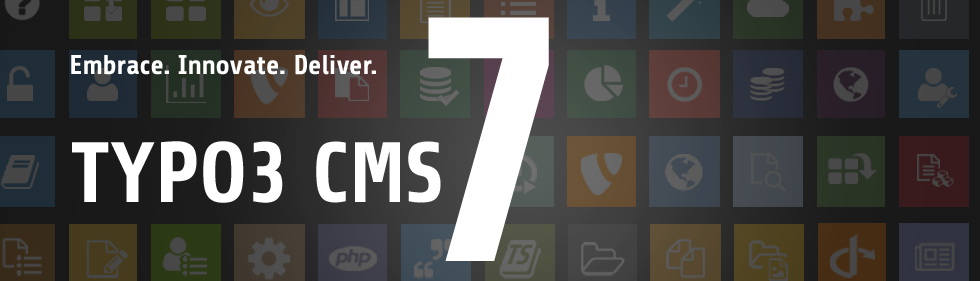
\includegraphics[width=0.95\linewidth]{typo3-seven-zero-banner.png}
	\end{figure}

\end{frame}

% ------------------------------------------------------------------------------
% LTXE-SLIDE-START
% LTXE-SLIDE-UID:		62f0c069-268cc7aa-a0147136-bf3b8c9c
% LTXE-SLIDE-ORIGIN:	f0c768bc-7a7f5fff-20ca5059-23f8e843 English
% LTXE-SLIDE-TITLE:		System Requirements
% ------------------------------------------------------------------------------

\begin{frame}[fragile]
	\frametitle{Введение}
	\framesubtitle{Системные требования}

	\begin{itemize}
		\item PHP*:\tabto{3.2cm}v5.5.0 - v5.6.x
		\item MySQL:\tabto{3.2cm}v5.5.x - v5.6.x (без strict mode)
		\item Место на диске:\tabto{3.2cm}мин. 200 MB
		\item Настройки PHP:

			\begin{itemize}
				\item memory\_limit >= 128M
				\item max\_execution\_time >= 240s
				\item параметр компиляции \texttt{--disable-ipv6} \underline{не} должен использоваться
			\end{itemize}

		\item Внутренний интерфейс требует IE >= 9 или любой современный браузер

	\end{itemize}

	\vspace{0.2cm}
	*) Детально: \href{http://typo3.org/news/article/php-minimum-requirements-for-typo3-cms-7/}{PHP Minimum Requirements for TYPO3 CMS 7}

\end{frame}

% ------------------------------------------------------------------------------
% LTXE-SLIDE-START
% LTXE-SLIDE-UID:		3a1c637e-0a243869-84a9cef9-5bc2549c
% LTXE-SLIDE-ORIGIN:	e6dd8a1b-2b60f76b-adc1d788-f77036d9 English
% LTXE-SLIDE-TITLE:		Development And Release Timeline
% ------------------------------------------------------------------------------

\begin{frame}[fragile]
	\frametitle{Введение}
	\framesubtitle{График разработки и выхода}

	\begin{figure}
		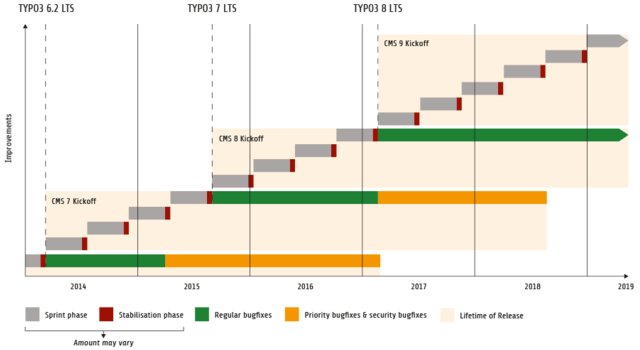
\includegraphics[width=0.90\linewidth]{Introduction/ReleaseAgenda.png}
	\end{figure}

\end{frame}

% ------------------------------------------------------------------------------
% LTXE-SLIDE-START
% LTXE-SLIDE-UID:		9621146c-3829db66-7baf009d-b50916a1
% LTXE-SLIDE-ORIGIN:	a99cfec1-0a35c0fb-e552ac34-e4e407f8 English
% LTXE-SLIDE-TITLE:		TYPO3 CMS Roadmap
% ------------------------------------------------------------------------------
% https://typo3.org/typo3-cms/roadmap/

\begin{frame}[fragile]
	\frametitle{Введение}
	\framesubtitle{TYPO3 CMS дорожная карта}

	Примерные даты выхода и их основной фокус:

	\begin{itemize}
		\item
			\smaller
				\begingroup
					\color{typo3orange}
						v7.0 \textrightarrow\tabto{1.3cm}02/Dec/2014\tabto{3.4cm}Переработка внутреннего интерфейса часть 1
				\endgroup
			\normalsize

		\item\smaller v7.1 \textrightarrow\tabto{1.2cm}17/Февр./2015\tabto{3.4cm}Чистка ядра и оптимизация\normalsize
		\item\smaller v7.2 \textrightarrow\tabto{1.2cm}10/Март/2015\tabto{3.4cm}Внешний интерфейс\normalsize
		\item\smaller v7.3 \textrightarrow\tabto{1.2cm}21/Апр./2015\tabto{3.4cm}Композитор экосистемы\normalsize
		\item\smaller v7.4 \textrightarrow\tabto{1.2cm}09/Июнь/2015\tabto{3.4cm}Переработка внутреннего интерфейса часть 2\normalsize
		\item\smaller v7.5 \textrightarrow\tabto{1.2cm}28/Июль/2015\tabto{3.4cm}\textit{(буедет уточнено...)}\normalsize
		\item\smaller v7.6 \textrightarrow\tabto{1.2cm}13/Окт./2015\tabto{3.4cm}пре-LTS инферно\normalsize
		\item\smaller v7.7 \textrightarrow\tabto{1.2cm}xx/xxx/2015\tabto{3.4cm}\textbf{TYPO3 CMS 7 LTS} (Long Term Release)\normalsize
	\end{itemize}

	\smaller
		\url{https://typo3.org/typo3-cms/roadmap/}\newline
		\url{http://typo3.org/news/article/embrace-and-innovate-typo3-cms-7/}
	\normalsize

\end{frame}

% ------------------------------------------------------------------------------
% LTXE-SLIDE-START
% LTXE-SLIDE-UID:		9bd83980-28ab4ccb-36dab401-d73591e0
% LTXE-SLIDE-ORIGIN:	185b2d64-63cab652-fa469322-8a16b1b7 English
% LTXE-SLIDE-TITLE:		Installation
% LTXE-SLIDE-REFERENCE:	https://forge.typo3.org/issues/62578
% ------------------------------------------------------------------------------

\begin{frame}[fragile]
	\frametitle{Введение}
	\framesubtitle{Установка}

	\begin{itemize}
		\item Официальная процедура установки под Linux/Mac OS X\newline
			(DocumentRoot например \texttt{/var/www/site/htdocs}):
		\begin{lstlisting}
			$ cd /var/www/site
			$ wget --content-disposition get.typo3.org/7.0
			$ tar xzf typo3_src-7.0.0.tar.gz
			$ cd htdocs
			$ ln -s ../typo3_src-7.0.0 typo3_src
			$ ln -s typo3_src/index.php
			$ ln -s typo3_src/typo3
			$ touch FIRST_INSTALL
		\end{lstlisting}

		\item Symbolic links под Microsoft Windows:

			\begin{itemize}
				\item Используйте \texttt{junction} под Windows XP/2000
				\item Используйте \texttt{mlink} под Windows Vista и Windows 7
			\end{itemize}

	\end{itemize}
\end{frame}

% ------------------------------------------------------------------------------
% LTXE-SLIDE-START
% LTXE-SLIDE-UID:		0c4bfacd-f52a24b3-351234d0-68a61558
% LTXE-SLIDE-ORIGIN:	d884c8cf-25261e85-a2a26fcd-8a64a9cb English
% LTXE-SLIDE-TITLE:		Upgrade to TYPO3 CMS 7 (1)
% LTXE-SLIDE-REFERENCE:	https://forge.typo3.org/issues/62578
% ------------------------------------------------------------------------------

\begin{frame}[fragile]
	\frametitle{Введение}
	\framesubtitle{Обновление до TYPO3 CMS 7.x}

	\begin{itemize}
		\item Обновление возможно лишь с TYPO3 CMS 6.2 LTS
		\item TYPO3 CMS < 6.2 должны быть обновлены сначала до TYPO3 CMS 6.2 LTS
	\end{itemize}

	\begin{itemize}

		\item Инструкции по обновлению:\newline
			\smaller\url{http://wiki.typo3.org/Upgrade#Upgrading_to_7.0}\normalsize
		\item Официальное руководство TYPO3 "TYPO3 Installation and Upgrading":
			\smaller\url{http://docs.typo3.org/typo3cms/InstallationGuide}\normalsize
	\end{itemize}

\end{frame}

% ------------------------------------------------------------------------------
% LTXE-SLIDE-START
% LTXE-SLIDE-UID:		xxxxxxxx-xxxxxxxx-xxxxxxxx-xxxxxxxx
% LTXE-SLIDE-ORIGIN:	xxxxxxxx-xxxxxxxx-xxxxxxxx-xxxxxxxx
% LTXE-SLIDE-TITLE:		Upgrade to TYPO3 CMS 7 (2)
% LTXE-SLIDE-REFERENCE:	https://forge.typo3.org/issues/62578
% ------------------------------------------------------------------------------

\begin{frame}[fragile]
	\frametitle{Введение}
	\framesubtitle{Обновление до TYPO3 CMS 7.x}

	\begin{itemize}
		\item Общий подход:
			\begin{itemize}
				\item Проверка минимальных системных требований \small(PHP, MySQL и т. п.)
				\item Просмотр \textbf{deprecation\_*.log} в старой версии TYPO3
				\item Обновление всех расширений до последней версии
				\item Загрузка новых исходных файлов и запуск Install Tool \textrightarrow Upgrade Wizard
				\item Запуск модуля обзора для внутренних пользователей (опционально)
			\end{itemize}
	\end{itemize}

\end{frame}

% ------------------------------------------------------------------------------
